The development of CubeSats started in 1999 with members of \ac{Cal Poly} and \ac{SSDL}. The nanosatellites' standard is $10\times 10\times 10$~\acs{cm}  with a maximum weight of 1.33~\acs{kg} (1U CubeSat) \cite{california_polytechnic_state_university_cubesat_2014}.
\newline
Their main field of application are educational experiments conducted by Universities for example in -situ observations of lower thermospheric waves \cite{sanchez_benefits_2007}, but because to their being relatively low priced anyone who can raise enough money can build one. In 2012 there was even a successfully funded Kickstarter-project \cite{ppl4world_ardusat_2012}.
\newline
Another feasible field of use could be Telemedicine. CubeSats could be used to obtain and send telemetry data from hard to reach sources. Moreover, in countries with a low density of medical experts, the CubeSats could be used to send the data to experts located far away. There they could be analyzed and sent back.
\newline
In 2007 the \textit{Universidad Distrital Francisco Jose de Caldas} proposed a plan to implement a telemedicine pilot project to transmitting and receiving ECG signals via CubeSats at \textit{The 2007 CubeSat Developer's Workshop}  \cite{pico_cubesat_2007}. A project like that could lead to a much better healthcare for a lot of people in developing countries.
\newline
Several companies research the use of smartphone processors as the central avionics in in high altitude leading to the first successfull launch of a CubeSat stocked with the processor of the HTC Nexus One by \ac{SSTL} \cite{surrey_satellite_technology_ltd._iac-11-b4.6b.8_2011} and later that year to the PhoneSat project of the \ac{NASA} where they used the processors of the HTC Nexus One and Samsung Nexus S \cite{attai_phonesat_2014}.
\newline
\begin{figure}[ht!]
\centering
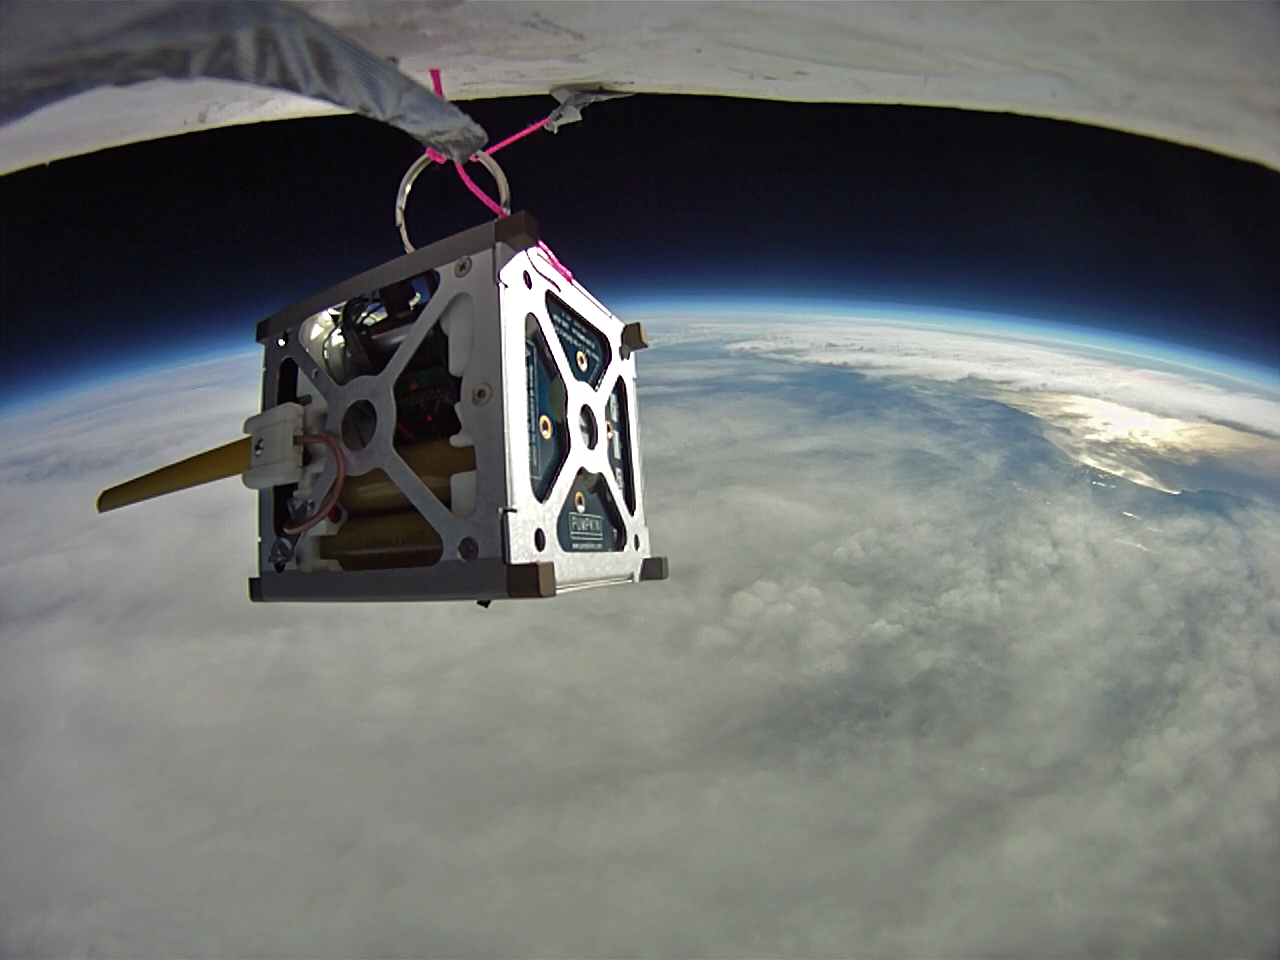
\includegraphics[width=120mm]{PICs/NASA_PhoneSat.jpg}
\caption[NASA PhoneSat \cite{jurvetson_nasa_2011}]{NASA PhoneSat - licensed under CC BY 2.0 \label{PhoneSat}}
\end{figure}
\newline
